% 1. Develop, test and deploy a new software workflow to incorporate external packages into Bonsai's C# environment.

% 2. Incorporate a suite of machine-learning-driven analysis tools into the Bonsai environment to implement:
% 2a. video-based  behavioural analysis
% 2b. real-time interfacing of population-scale activity with laboratory control  
% 2c. evaluate competing data analytic approaches within a single experimental framework

\section{Details of proposed resource enhancements}

We will enhance Bonsai's extensibility in two ways.
%
First, we will create a new package infrastructure to enable the integration of software objects implemented in non-native languages into Bonsai.
%
Second, we will create a new general abstraction framework within Bonsai suited to the implementation and application of data analytic algorithms.
%
Both frameworks will expose public interfaces available to all developers within the user community, thus simplifying and accelerating community-driven development.

Furthermore, we will build on these extensibility developments to implement a suite of advanced machine intelligence neural data analysis methods that will be made available as one or more core Bonsai packages.

\subsection{Extensions to incorporate non-native code packages into Bonsai}

Bonsai is designed to be extensible and is distributed with a package-management framework that controls installation of optional core packages as well as user-contributed extensions.
%
However, extensions must be written in Bonsai's native C\# programming language.
%
This restricts the range of potential contributors to the ecosystem.
%
It also hinders incorporation of published analytic tools, many of which are implemented within other interpreted language systems such as Python, R, or MATLAB.  
\begin{wrapfigure}{R}{0pt}
  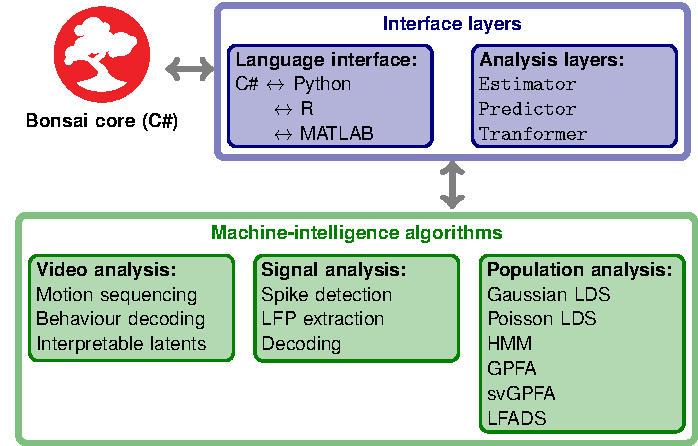
\includegraphics[width=0.5\textwidth]{figures/extensions.pdf}%
%   % \documentclass{standalone}
% %% Fonts, etc.

% %% Language and font encodings
% \usepackage[english]{babel}
% \usepackage[utf8x]{inputenc}
% \usepackage[T1]{fontenc}

%  \usepackage[scaled=0.92]{helvet} \renewcommand{\familydefault}{\sfdefault}
%  \usepackage{xcolor}
% % \usepackage{soul} % \ul \st \hl


% %% Maths

% % \usepackage{amssymb,amsmath}
% % \input m.macros
% % \input m.symbols


% %% Graphics

% \usepackage{graphicx,tikz}
% \usetikzlibrary{positioning}
% \usetikzlibrary{fit}
% \usetikzlibrary{calc}






% %% Document
% \begin{document}

\begin{tikzpicture}[
    ML/.style={text width=10em, rounded corners,
      fill=green!50!black!30, draw=green!50!black, very thick},
    Ext/.style={text width=10em, rounded corners,
      fill=blue!50!black!30, draw=blue!50!black, very thick}
    ]

  \node[text width=10em, font={\bf}, align=center]
       (bonsai)
       {\includegraphics[width=7em]{bonsai-lettering}\\
         Bonsai core (C\#)};

       
 \coordinate [below = 5em of bonsai.south] (A);

  \node[below left=0 and 1em of A, Ext]
       (lang)
       {\textbf{Language interface:}\\
         C\# $\leftrightarrow$ Python\\
         $\qquad \leftrightarrow$ R\\
         $\qquad \leftrightarrow$ MATLAB
       };


  \node[below right=0 and 1em of A, Ext]
       (abstr)
       {\textbf{Analysis layers:}\\
         \texttt{Estimator}\\
         \texttt{Predictor}\\
         \texttt{Tranformer}};

  \node[above=1ex of A, text=blue!50!black, font={\bf}, inner sep=0]  (intr) {Interface layers};

  \node[fit=(lang) (abstr) (intr), line width=1mm, draw=blue!50!black!50, rounded
    corners, inner sep=1ex] (intr box) {};

 \coordinate [below = 12em of A] (B);


 \node[below=0 of B, ML]
       (signal)
       {\textbf{Signal analysis:}\\
         Spike detection\\
         LFP extraction\\
         Decoding};

  \node[below left=0 and 1em of signal.north west, ML]
       (video)
       {\textbf{Video analysis:}\\
         Motion sequencing\\
         Behaviour decoding\\
         Interpretable latents};
       
       
  \node[below right=0 and 1em of signal.north east, ML]
       (dimred)
       {\textbf{Population analysis:}\\
         Gaussian LDS\\
         Poisson LDS\\
         HMM\\
         GPFA\\
         svGPFA\\
         LFADS};

  \node[above=1ex of B, text=green!50!black, font={\bf}, inner sep=0] (ml)
       {Machine-intelligence algorithms};

  \node[fit=(video) (signal) (dimred) (ml), line width=1mm, draw=green!50!black!50, rounded
    corners, inner sep=1ex] (ml box) {};


  \draw[<->, line width=1mm, gray] (bonsai) -- (intr box);

  \draw[<->, line width=1mm, gray] (intr box) -- (ml box);

  
  

  %% \node[below = 15em of bonsai, ML]
  %% (compare)
  %%      {\textbf{Method comparison}};
       
\end{tikzpicture}

% \end{document}

% Local Variables:
% mode: latex
% eval: (set-fill-column 80)
% End:

  \caption{Proposed extensions to Bonsai}
  \label{fig:proposedBonsaiExtensions}
\end{wrapfigure}

We will extend the Bonsai package interface to allow direct interaction with the runtime execution environments that implement these common languages.  
%
Where possible, the extensions will be based on existing pipeline tools that allow C\#-based programs to interact with a number of alternative run-time engines.
%
These include:
%
Python.NET\footnote{https://github.com/pythonnet/pythonnet},
%
R.Net\break \footnote{https://github.com/rdotnet/rdotnet}
%
and the native .NET interface shipped with MATLAB.
% \footnote{https://uk.mathworks.com/help/matlab/matlab\_external/using-net-from-matlab-an-overview.html}.  TOO LONG
%
If necessary, we will also incorporate direct inter-runtime communication using the messaging library ZeroMQ\footnote{https://zeromq.org/}.

\subsection{General abstraction framework for data processing}
\label{sec:generality}

To avoid the need to re-implement a single data analysis algorithm to handle multiple different data types we will create a set of abstract machine-intelligence operators in Bonsai that can be configured to map between data substrates and ML algorithms.
%
The planned abstraction layer is based on the successful \texttt{scikit-learn} Python
library \citep{buitinckEtAl13}.
%
By analogy to the interfaces provided by this library we will introduce three types of Bonsai operator: \texttt{Estimator} objects for building and fitting models, \texttt{Predictor} objects for making predictions and \texttt{Transformer} objects for converting data.
%
Interactions between these different object types will allow a single algorithm class (implemented by \texttt{Estimator} and \texttt{Predictor} operators) to act on many different data streams.
%
% An example closed-loop architecture allowing online control of a compu|ter cursor with neural activity is shown in Figure~\ref{fig:proposedBonsaiExtensions}b. The Bonsai
% graphical program for this system is given in Figure~\ref{fig:proposedBonsaiExtensions}c. The
% objects instantiating the SpikeThresholdDetector, the KiloSortSpikeSorter and
% GPFAlatentsExtractor implement the \texttt{Transformer} interface (blue),
% and the object instantiating the TimeSeriesForestClassifier implements the
% \texttt{Predictor} interface (green; Figure~\ref{fig:proposedBonsaiExtensions}c, top).
% %
% While the parameters for the SpikeThresholdDetector and the KiloSortSpikeSorter may
% be set manually by the user, the parameters of
% the GPFAlatentsExtractor can be learnt offline in an unsupervised way using an
% \texttt{Estimator} (red) in a second pipeline
% (Figure~\ref{fig:proposedBonsaiExtensions}c, middle).
% Finally, the parameters of the TimeSeriesForestClassifier can also be learnt
% offline, but in a supervised way, using another \texttt{Estimator} in a third
% pipeline (Figure~\ref{fig:proposedBonsaiExtensions}c, bottom).






% This initial set of methods should demonstrate to Bonsai users, and to
% machine-learning methods developers, the potential of embedding
% machine-learning functionality into the experimental control loop. We propose
% user engagement activities to expose both of these groups to this
% potential (Section~\ref{sec:userEngagement}).  As data-analysis method
% developers recognise this opportunity, they will become interested in
% contributing their methods to the Bonsai ecosystem, ensuring the
% \textbf{long-term sustainability} of the proposed resource.

% Adding machine learning functionality to the experimental control loop will
% make possible the implementation of experiments with unprecedented levels of
% control. Moreover, equipping experimental scientists without programming
% experience with machine learning tools will considerably increase the
% application of machine learning to the biosciences, which most probably will
% translate into groundbreaking scientific discoveries.



% Developers of advanced data-analysis methods should become interested in
% integrating them into the Bonsai ecosystem, as it will allow their methods to
% reach the wide Bonsai user community. In addition this integration will enable
% method developers to easily compare the performance of their methods with
% that of many methods previously integrated into the Bonsai ecosystem. Method
% developers will thus become a new type of Bonsai users, which will contribute
% to the \textbf{sustainability} of the proposed resource beyond the period of
% BBSRC-BBR funding.

% Scientific advances rely on \textbf{reproducibility}, which in turn depends on standardized tools for experimental control and analysis, shared between laboratories (Baker, 2016; Ioannidis, 2005). Although such tools exist in genetics, astronomy, physics and medicine (Fish et al., 2016; Abdalla et al., 2018, CERN Education, Communications and Outreach Group, 2018, Dickinson et al., 2016, Bycroft et al., 2018), they are mostly lacking in neuroscience, which in itself suffers from a paucity of reproducible discoveries (Baker, 2016; Botvinik-Nezer et al., 2020; Button et al., 2013). Bonsai is an excellent tool for reproducible data acquisition and experimental control. For example, an experiment implemented in Bonsai can be replicated in
% any laboratory by just sharing a Bonsai configuration file. With the addition of the proposed machine learning functionality Bonsai will extend this
% reproducibility to the domain of data analysis
% (Section~\ref{sec:reproducibility}).


% \begin{figure} \begin{center}

%     \href{http://www.gatsby.ucl.ac.uk/~rapela/bbsrc-bbr21/proposed_bonsai_extensions_combined.png}{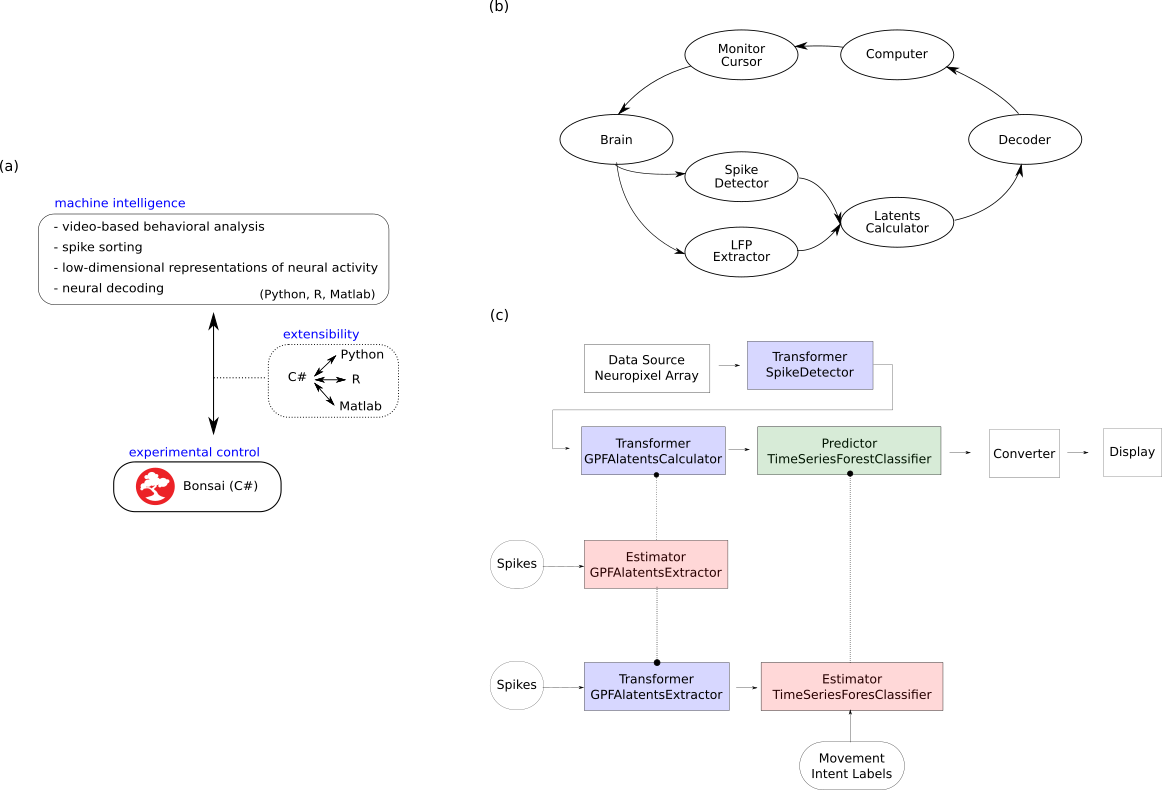
\includegraphics[width=5in]{figures/proposed_bonsai_extensions_combined.png}}

%     \caption{Extensions to Bonsai. (A) we propose to integrate machine learning
%     functionality into the experimental control loop by building software
%     infrastructure to allow Bonsai to communicate with existing machine
%     learning software written in Python, R and Matlab. (B) flow chart
%     representing the BCI application that we propose to implement with the
%     machine learning functionality to be added to Bonsai. (C) Bonsai graphic
%     program implementing the BCI application in (B).}

%         
%     \end{center}
% \end{figure}


\subsection{Machine intelligence functionality}
\label{sec:functionality}

We will use the frameworks developed above to integrate existing machine-intelligence programs within one or more Bonsai packages.  Based on user input, we have identified initial domains of video-based behavioural analysis (Section~\ref{sec:videoBasedBehavioralAnalysis}) and
brain-computer-interface (BCI) experiments (Section~\ref{sec:bci}). 

\subsubsection{Video-based behavioural analysis}
\label{sec:videoBasedBehavioralAnalysis}

Precisely quantifying animal behaviour is an essential step toward understanding
brain function.  DeepLabCut is a Python-based software for tracking animal body
parts \citep{mathisEtAl18}, which is currently well integrated with
Bonsai~\citep{kaneEtAl20}. Here we propose extensions to Bonsai to extract
other informative features from video recordings.

\begin{description}

    \item[Motion sequencing]\citep[MoSeq;][]{wiltschkoEtAl15}: extracts patterns
        of behaviour that repeat over time (i.e., syllables of behaviour) from
        video data. For instance, it parses (in an unsupervised way) the
        behaviour of a mouse in an arena into segments of time where a mouse
        was running, rearing and grooming. It uses a hidden Markov model and it
        is implemented in Python\footnote{Code for MoSeq can be requested from
        the Datta laboratory, as indicated at
        http://datta.hms.harvard.edu/research/behavioral-analysis/.}.
        After trained MoSeq can be used to detect behavioural syllables online.

    \item[Decoding behaviour from neural
        activity]\citep[BehaveNet;][]{battyEtAl19} combines hidden Markov
        models with convolutional autoencoders and discriminative models to
        decode video data from neural recordings. It is implemented in
        Python\footnote{https://github.com/themattinthehatt/behavenet}.
        After trained it can be used online to decode video data and detect
        behavioral syllables.

    \item[Interpretable latents for behavioral videos]\citep[Partitioned
        Subspace Variational Autoencoder, PS-VAE;][]{whitewayEtAl21}: produces
        interpretable low-dimensional representations of behavioral videos by
        combining the output of pose-estimation algorithms (e.g., DeepLabCut)
        with unsupervised dimensionality reduction methods. These
        low-dimensional representations facilitate downstream behavioral and
        neural analyses. It is based on autoencoders and is implemented in
        Python\footnote{code for PS-VAE is embedded in the BehaveNet code
        https://github.com/themattinthehatt/behavenet.%
        % Please refer to class \texttt{PSVAE} in texttt{behavenet.models.vaes.py}.
        }. After trained it can be used
        online to extract low-dimensional features and perform downstream
        processing.

\end{description}

\subsubsection{Brain-computer-interface applications}
\label{sec:bci}

We propose to add functionality into Bonsai for the implementation of
brain-computer-interface (BCI) applications illustrated in
Figure~\ref{fig:proposedBonsaiExtensions}b. In
this implementation voltage recordings from the brain will be converted into
spikes fired by single neurons by a \texttt{SpikeDetector}
(Section~\ref{sec:spikeDetection}), or to local field potentials (LFP) by an
\texttt{LFPextractor} (Section~\ref{sec:lfpExtraction}). Next, neural activity
(spikes or LFPs) will be represented in a low-dimensional latent space by a
\texttt{LatentsCalculator}. Finally, a \texttt{Decoder} will extract the
intended behaviour of the animal from this low-dimensional representation.

\paragraph{Spike detection}
\label{sec:spikeDetection}

Spikes from multiple neurons can be detected in recordings from a single
electrode inserted in neural tissue. Spike sorting is the computational step
used to assign each spike to the neuron that generated it. Most spike sorting
algorithms are designed to work offline (i.e., to use a complete recording
session, after this session terminated). Online spike sorting (i.e., the task
of assigning spikes to individual neurons as recordings are being aquired) is a
still unsolved task, specially for recording devices with large number of
electrodes.
%
However, for the type of BCI application proposed here, previous studies have
shown that spike sorting is not beneficial and high performance can be retained
by just detecting spikes, without assigning them to invidivual
neurons~\citep{trautmannEtAl19,todorovaEtAl14}. Thus, for the BCI application
proposed here we will only detect spikes with a simple zero-corssing method,
and not assign them to individual neurons.  We will, however, integrate into
Bonsai two offline spike sorting methods, Kilosort~\citep[][written in Matlab]{pachitariuEtAl16} and MountainSort~\citep[][written in
Python]{chungEtAl17}, to provide Bonsai users spike sorting functionality for
applications that benefit from it.

\paragraph{LFP extraction}
\label{sec:lfpExtractor}

Spikes are extracted from a higher-frequency range of extracellularly recorded
voltages. Local field potentials (LFPs) 
are another important signal to understand brain function, which is extracted
from a lower-frequency range of these voltages. We propose to use in-house
functions implemented in Python to compute LFPs.

\paragraph{Low-dimensional representations of neural recordings}
\label{sec:lowDimensionalRepresentation}

Bonsai is well integrated with OpenEphys~\citep{siegleEtAl17}, which allows
scientists to record neural data from a large number of devices. However, it
lacks functionality to process these recordings. Here we describe software that
we propose to integrate into Bonsai to extract interpretable summary statistics
(i.e., latent variables) from neural spiking activity.

\begin{description}

    \item[Gaussian Linear Dynamical
        System]\citep[GLDS][]{andersonAndMoore12}: with sufficiently large
        bin sizes, spike counts can be modelled as Gaussian random processes.
        This Gaussianity assumption greatly simplifies the estimation of
        parameters of linear dynamical system (LDS) models, as well as
        inferences about their states. After models parameters have been
        learned, GLDS can be used online. A unique feature of GLDS is that the
        posterior distribution of states given all observation up to the
        present can be calculated efficiently. This estimate of the posterior
        distribution can be used online for experimental control, as we
        propose in Section~\ref{sec:comparisonOfMultipleMethods}. We will use an R implementation of GLDS
        which allows the use of external
        inputs\footnote{https://github.com/joacorapela/kalmanFilter}.

    \item[Poisson Linear Dynamical System]\citep[PLDS][]{mackeEtAl15}: for
        smaller bin sizes, spike counts are better modelled as Poisson random
        processes, rather than Gaussian ones. The algorithm described in
        \citet{mackeEtAl15} can estimate the parameters of a LDS, and make
        inferences about its states, from Poisson distributed observations.  We
        propose to interface Bonsai with a Matlab implementation of
        PLDS\footnote{https://bitbucket.org/mackelab/pop\_spike\_dyn/src/master/}
        that uses variational inference. PLDS does not provide online estimates
        of the states, since data from a full trial is needed for state
        inference.

    \item[Hidden Markov Model]\citep[HMM;][]{rabiner89}: as LDSs, HMMs model a
        time series of observations as random processes conditioned on hidden
        states. However, in HMMs hidden states are discrete random variables,
        while in LDSs they are continuous ones. In some application domains
        (e.g., speech, epilepsy) discrete state assumptions are more pertinent
        than continuous ones. We propose to use an R implementation of
        HMMs\footnote{https://github.com/joacorapela/hiddenMarkovModels}.
        As GLDSs, once trained, HMMs can be used online to infer the posterior
        distribution of states given observations.

    \item[Gaussian Processes Factor Analysis]\citep[GPFA;][]{yuEtAl09}: as
        LDSs, GFPA models represent a time series of observation as random
        processes conditioned on hidden states. However, in GPFA models the
        state dynamics are nonlinear, while in LDS models they are linear.
        Thus, GPFA models are more general than LDS ones. As GLDS models, GPFA
        models assume that observations conditioned on states are Gaussian
        random processes. We propose to use a Matlab implementation of
        GPFA\footnote{https://users.ece.cmu.edu/~byronyu/software/gpfa0203.tgz}.
        GPFA models do not provide online estimates of the states, since data
        from the full trial are needed for state estimates.

    \item[Sparse Variational Gaussian Processes Factor
        Analysis]\citep[svGPFA;][]{dunckerAndSahani18}: is similar to GPFA, but
        models point process observations (i.e., single spikes as opposed to
        spike counts). We propose to use a Python implementation of
        svGPFA\footnote{https://github.com/joacorapela/svGPFA}.
        svGPFA models do not provide online estimates of states, since data
        from the full trial are needed for state estimates.

    \item[Latent factor analysis through dynamical
        systems]\citep[LFADS;][]{pandarinathEtAl18}: uses an autoencoder
        framework, with recursive neural networks, to infer continuous states
        conditioned on spike counts, similar to those inferred by GPFA. We
        propose to use a Python implementation at
        LFADS\footnote{https://github.com/tensorflow/models/tree/master/research/lfads.}.
        As GPFA, LFADS do not provide online estimates of states.

\end{description}

\paragraph{Low-dimensional representations of local-field potentials}
\label{sec:lowDimensionalRepresentationsOfLFPs}

Spikes are extracted from a higher-frequency range of extracellularly recorded
voltages. Local field potentials (LFPs) are computed from a lower-frequency
range and are another important signal to understand brain function. We propose
to use states inferred from LFPs by GLDS, GPFA, HMM and LFADS
(Section~\ref{sec:lowDimensionalRepresentation}) as
low-dimensional representations of the LFP.

\paragraph{Neural decoding}
\label{sec:neuralDecoding}

In order to use low-dimensional representations of spiking activity and/or of
LFPs to guide the control of experiments, we need a decoder to optimally map
these low-dimensional representations to experimental controls.
%
We propose to implement in Bonsai several decoding/classification algorithms:
k-nearest neighbour, linear discriminative analysis, support vector machines,
random forests, artificial neural networks, naive Bayes and Gaussian process
classifiers.

\subsection{Comparing multiple data-analysis methods}
\label{sec:comparisonOfMultipleMethods}

We propose to add functionality to Bonsai to facilitate multi-method
comparisons in user-supplied datasets.

% Below we describe a comparison that we
% will perform in Bonsai to asses the relative performance of the methods
% described in the previous sections, using neural recordings from behaving rats.
% These recordings are currently being performed, to address scientific questions,
% at the laboratory of Prof.~Akrami in the SWC.
% %
% Details of the experimental task appear in~\citet{akramiEtAl18}.
% %
% Briefly, in this task there are three nose ports (left, centre, right). Rats
% initiate a trial by inserting their nose in the centre port for the duration of
% the fixation period, until they hear a Go stimulus. During the fixation period
% two stimuli $s_a$ and $s_b$ are presented. Rats should decide which stimuli is
% louder. If $s_a$ is louder than $s_b$ the correct action is to poke the nose
% into the right port in order to collect a liquid reward, and if $s_b$ is louder
% than $s_a$ the correct choice is the left port.

% We will use high-density Neuropixel spike and LFP recordings from the rats
% performing this task to learn low-dimensional representations of spiking
% activity and LFPs during the decision time period (between the presentation of
% the last auditory stimuli and the presentation of the Go stimulus), using the
% methods described in
% Sections~\ref{sec:lowDimensionalRepresentation}
% and~\ref{sec:lowDimensionalRepresentationsOfLFPs}. We will also learn the
% parameters of the classifiers described in Section~\ref{sec:neuralDecoding} to
% optimally classify animal decisions (poke the nose into the right/left port)
% based on the previous low-dimensional representations.

% We will compare the decoding accuracy of all decoders. This comparison will
% tells us, for the auditory working memory task, which neural data type (spikes
% or LFPs), which low-dimensional representation method (e.g., LDS or Gaussian
% processes), and which decoder (e.g., Bayesian or ANN) yields the best decodings
% in state-of-the-art neural recordings from behaving animals.

\begin{comment}

\subsection{Interfacing Bonsai with Python, R and Matlab data analysis software}
\label{sec:bonsaiPythonMatlabCommunication}

Bonsai is written in C\# and most neural data-analysis methods are written in
Python, R or Matlab. Fortunately, there exist software that allow C\# program
to call and be called by programs in these other languages. For the
communication of C\# programs with Python we will use
Python.NET\footnote{https://github.com/pythonnet/pythonnet},
with R programs we will use
R.Net\footnote{https://github.com/rdotnet/rdotnet}
and with Matlab we will use the built in Matlab .NET
interface\footnote{https://uk.mathworks.com/help/matlab/matlab\_external/using-net-from-matlab-an-overview.html}.
In cases where these software cannot support some type of communication between
C\# and another language we will use the messaging library
ZeroMQ\footnote{https://zeromq.org/}.

\end{comment}

\subsection{Testing with neuroscience data}
\label{sec:testingWithNeuroscienceData}

Multiple groups at the SWC currently use Bonsai for data acquisition and
experimental control. Carefully testing the functionality of new software is
essential to ensure its correct functionality. We propose to use the SWC large
internal Bonsai user base to test the functionality we will add to Bonsai,
before distributing it to the general public.

\subsection{Reproducibility with Bonsai}
\label{sec:reproducibility}

The current version of Bonsai facilitates reproducibility of data acquisition
and experimental control across laboratories. Most data acquisition and
experimental control aspects of an experiment can be reproduced across
different laboratories by sharing a Bonsai configuration file.
%
By adding data analysis functionality to Bonsai, besides reproducing my data
acquisition and experimental control, Bonsai users will also be able to reproduce
data analysis functionality.

We will demonstrate each machine intelligence functionality added to Bonsai
(Section~\ref{sec:functionality}) and the multiple
data-analysis methods comparisons
(Section~\ref{sec:comparisonOfMultipleMethods}) in Bonsai experiments. We will
then distribute Bonsai configuration files for users to reproduce these
demonstrations.

\subsection{Measurable targets}
\label{sec:measurableTargets}

We propose to assess the progress of the proposed project using three different
types of targets.
%
First, we will have targets associated with each release to the general public
of the software components described above. 
% in Sections~\ref{sec:infrastructure} and~\ref{sec:functionality}.
%
Second, we will monitor user activity in the Bonsai
forum\footnote{https://groups.google.com/g/bonsai-users},
and publications citing Bonsai that use the new ML functionality,
to estimate the number of Bonsai users using this functionality.
%
Third, we will count the number of ML methods that are integrated
into the Bonsai ecosystem by us and by other method developers.

\begin{comment}

\begin{description}

    \item[implementation of software infrastructure]
        (Section~\ref{sec:infrastructure}) includes the
        implementation of the machine abstractions, described in
        Section~\ref{},
        and of the capabilities to allow Bonsai communicate with
        software written in other languages, described in Section~\ref{}. We
        will consider this target completed when we can implement a simple BCI
        application, with the architecture depicted in Figure~\ref{}, with
        machine learning functionality provided by software in Python, Matlab
        and R.

    \item[implementation of functionality] (Sections~\ref{sec:functionality})
        includes the integration into Bonsai of machine learning software for
        video-based behavioral analysis (Section~\ref{}) and for
        BCI applications (Section~\ref{}). Completion of
        this target requires that Bonsai can perform each of these tasks
        separately, in conjunction with software written in Python, R and
        Matlab.

    \item[internal testing] multiple groups at the SWC use Bonsai to control
        their experiments. 

        Bonsai Github repository and the success use by Bonsai users

    \item Bonsai users use the implemented machine learning functionality. We
        propose to evaluate this target by checking in the Bonsai user forum
        the frequency with which a novel machine learning functionality is
        discussed, and by tracking publications using this functionality.

    \item method developers integrate their methods into the Bonsai ecosystem.
        The integration of machine learning functionality into Bonsai will use
        Bonsai's package manager. We propose to use this package manager to tack
        the number of machine intelligence methods integrated into Bonsai.

\end{description}

\end{comment}

\begin{comment}

\subsection{Final remarks}
\label{sec:finalRemarks}

We proposed to add machine intelligence functionality to Bonsai to assist users
in building close-loop neural experiments: online spike sorting, methods for
low-dimensional representation of spiking activity and LFPs, and neural
decoding algorithms. This functionality will allow neuroscience Bonsai users to
build more sophisticated experiments and extract more information from their
experimental recordings.

We also proposed to add functionality to help Bonsai users compare the
performance of multiple methods on their datasets. With this functionality
Bonsai users will be able to select the best methods to model their own
recordings. It will also motivate methods developers to interface their
data-analysis functionality with Bonsai. By doing so, they will provide their
software to the large community of Bonsai users, and will be able to easily
compare the performance of their methods with that of preexisting methods in
the Bonsai ecosystem. In this way method developers will become a new type of
Bonsai users, which will guarantee the sustainability of developments
proposed here.

\end{comment}
